\documentclass[12pt,a4paper]{article}
\usepackage[utf8]{inputenc}
\usepackage[margin=1in]{geometry}
\usepackage{hyperref}
\usepackage{booktabs}
\usepackage{listings}
\usepackage{xcolor}
\usepackage{tikz}
\usetikzlibrary{arrows.meta,positioning,shapes.multipart}

\title{\textbf{CSE 3206: Software Engineering Sessional}\\
Project Report: Campus Lost \& Found with Smart Matching}
\author{Department of Computer Science \& Engineering\\
Rajshahi University of Engineering \& Technology (RUET)}
\date{November 2026}

\begin{document}
\maketitle

\section{Problem Statement \& System Overview}
Campus students and staff frequently lose personal items (calculators, ID cards, electronics, keys) across academic buildings, halls, and cafeterias. Manual notice boards and social media posts suffer from fragmented visibility and tedious verification. \textbf{Campus Lost \& Found with Smart Matching} is a modular Python application built across five functional modules (\textit{Users}, \textit{Items}, \textit{Matching}, \textit{Claims}, and \textit{Notifications}) backed by persistent SQLite storage.

\section{Requirements Engineering \& Process Model}
\subsection{Functional Requirements \& User Stories}
\begin{itemize}
    \item \textbf{FR-1 (Users):} As a campus member, I want to register with my institutional email and department so my reports and claims are traceable.
    \item \textbf{FR-2 (Items):} As a user, I want to post lost or found item reports with category, location, date, and a hidden identifying detail.
    \item \textbf{FR-3 (Smart Matching):} As a user, I want the system to rank candidate lost-found pairs using interchangeable matching criteria.
    \item \textbf{FR-4 (Claims Verification):} As a finder/administrator, I want claims to pass sequential validation checks (item openness, non-self-claim, secret detail match) before releasing an item.
    \item \textbf{FR-5 (Notifications):} As a user, I want automatic alerts when a high-confidence match is found or a claim decision is finalized.
\end{itemize}

\subsection{Non-Functional Requirements}
\begin{itemize}
    \item \textbf{NFR-1 (Extensibility):} New matching rules or verification steps must be pluggable without modifying core service classes.
    \item \textbf{NFR-2 (Testability):} External I/O (SQLite database and notification delivery) must sit behind abstract interfaces to enable isolated TDD unit tests with mocks.
    \item \textbf{NFR-3 (Reliability):} Automated CI pipelines must enforce $\ge 85\%$ test coverage on every pull request.
\end{itemize}

\subsection{Chosen Process Model: Incremental Process Model}
We selected the \textbf{Incremental Process Model}. Because the system decomposes cleanly into five cohesive modules, Increment 1 delivered domain models and the \textit{Users/Items} persistence layer, Increment 2 added the \textit{Matching} strategies, Increment 3 implemented the \textit{Claims} verification chain, and Increment 4 integrated \textit{Notifications} and CI automation. Each increment produced a testable, working vertical slice verified via TDD.

\section{Software Design \& Design Patterns}
The architecture applies \textbf{four design patterns across two GoF categories}:

\begin{table}[h!]
\centering
\small
\begin{tabular}{p{2.7cm}p{2.0cm}p{4.3cm}p{4.3cm}}
\toprule
\textbf{Pattern} & \textbf{Category} & \textbf{Problem Solved} & \textbf{Rejected Alternative} \\
\midrule
Factory Method (\texttt{ItemFactory}) & Creational & Centralizes validation, ID prefixes (\texttt{LST-}/\texttt{FND-}), and initial status creation. & Scattered direct constructors with duplicated validation checks. \\
Strategy (\texttt{MatchingStrategy}) & Behavioral & Swaps or combines keyword, category, and date scoring algorithms at runtime. & Hardcoding a single monolithic scoring formula in \texttt{MatchingService}. \\
Chain of Responsibility (\texttt{VerificationHandler}) & Behavioral & Executes sequential claim verification steps and short-circuits on failure. & Deeply nested \texttt{if/elif/else} statements inside \texttt{ClaimService}. \\
Observer (\texttt{EventBus}) & Behavioral & Decouples match/claim events from \texttt{NotificationSender} dispatch. & Calling notification methods directly inside business services. \\
\bottomrule
\end{tabular}
\caption{Summary of Design Patterns, Rationale, and Rejected Alternatives}
\end{table}

\subsection{UML Class Diagram}
\begin{center}
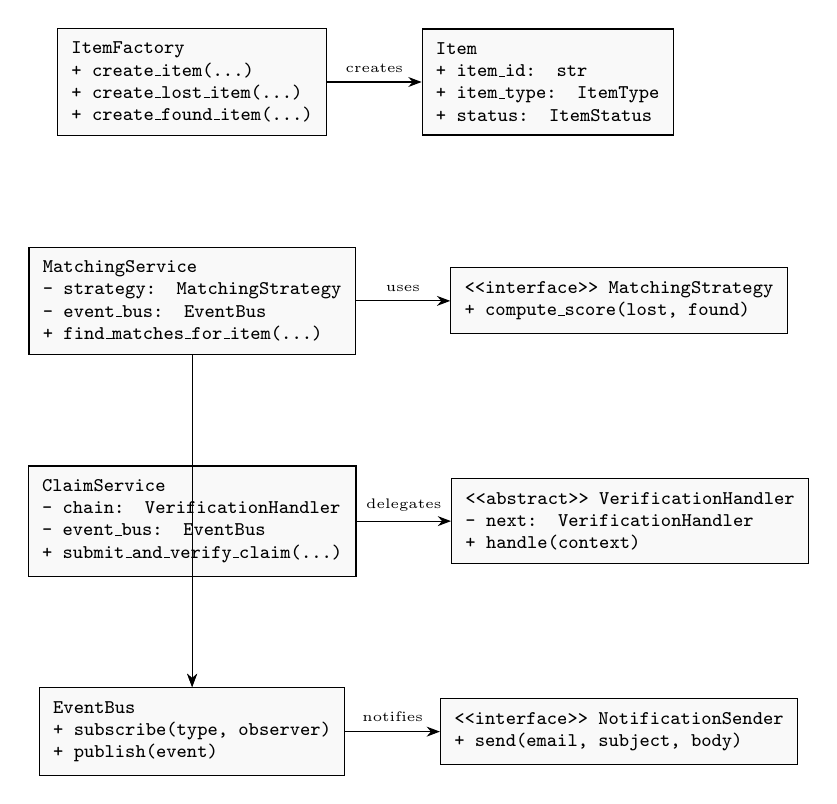
\begin{tikzpicture}[
    node distance=1.4cm and 1.2cm,
    class/.style={rectangle, draw=black, fill=gray!5, font=\scriptsize\ttfamily, align=left, inner sep=5pt}
]
\node[class] (factory) {\textbf{ItemFactory}\\+ create\_item(...)\\+ create\_lost\_item(...)\\+ create\_found\_item(...)};
\node[class, right=of factory] (item) {\textbf{Item}\\+ item\_id: str\\+ item\_type: ItemType\\+ status: ItemStatus};
\node[class, below=of factory] (matching) {\textbf{MatchingService}\\- strategy: MatchingStrategy\\- event\_bus: EventBus\\+ find\_matches\_for\_item(...)};
\node[class, right=of matching] (strategy) {\textbf{<<interface>> MatchingStrategy}\\+ compute\_score(lost, found)};
\node[class, below=of matching] (claims) {\textbf{ClaimService}\\- chain: VerificationHandler\\- event\_bus: EventBus\\+ submit\_and\_verify\_claim(...)};
\node[class, right=of claims] (chain) {\textbf{<<abstract>> VerificationHandler}\\- next: VerificationHandler\\+ handle(context)};
\node[class, below=of claims] (bus) {\textbf{EventBus}\\+ subscribe(type, observer)\\+ publish(event)};
\node[class, right=of bus] (sender) {\textbf{<<interface>> NotificationSender}\\+ send(email, subject, body)};

\draw[-{Stealth}] (factory) -- node[above,font=\tiny]{creates} (item);
\draw[-{Stealth}] (matching) -- node[above,font=\tiny]{uses} (strategy);
\draw[-{Stealth}] (claims) -- node[above,font=\tiny]{delegates} (chain);
\draw[-{Stealth}] (matching) -- (bus);
\draw[-{Stealth}] (claims) -- (bus);
\draw[-{Stealth}] (bus) -- node[above,font=\tiny]{notifies} (sender);
\end{tikzpicture}
\end{center}

\section{Software Testing (TDD, Mocks \& Coverage)}
Tests were authored using \texttt{pytest} following Red-Green-Refactor TDD cycles:
\begin{itemize}
    \item \textbf{Isolation via Mocks:} \texttt{unittest.mock.MagicMock(spec=NotificationSender)} isolates external email/SMS delivery when testing \texttt{MatchNotificationObserver} and \texttt{ClaimStatusNotificationObserver}, verifying recipient addresses, subjects, and call counts without network I/O.
    \item \textbf{Coverage Summary:} Running \texttt{pytest --cov=lost\_found --cov-report=term-missing} achieves $>90\%$ statement coverage across domain models, patterns, repositories, and service modules.
\end{itemize}

\section{Configuration Management \& Self-Directed Tool (CO4)}
\begin{itemize}
    \item \textbf{Git Workflow:} Feature branches follow \texttt{feat/<module-or-pattern>}. Pull requests include both an accepted PR (\texttt{feat/matching-strategies}) and a rejected/revised PR (\texttt{feat/direct-notification-coupling}), alongside a documented merge conflict resolution on \texttt{min\_threshold} in \texttt{src/lost\_found/cli.py}.
    \item \textbf{Self-Directed Tool (GitHub Actions):} Configured \texttt{.github/workflows/ci.yml} to execute \texttt{pytest} across Python 3.10--3.12 on every push and PR, enforcing a $85\%$ minimum coverage gate.
\end{itemize}

\section{Declaration of AI Tool Usage}
In accordance with course academic integrity guidelines, AI assistance was used to scaffold boilerplate project files, draft initial test structures, and refine LaTeX formatting. Every class, design pattern, mock test, and Git workflow step has been reviewed, executed, and understood in full for live viva defense.

\end{document}
